\setcounter{definition}{0} \setcounter{property}{0} \setcounter{claim}{0} \setcounter{fact}{0} \setcounter{corollary}{0} \setcounter{figure}{0}
\section{Shortest Path Tree}

So far we have designed three algorithms, BFS, Dijkstra's algorithm, and Bellman-Ford algorithm
to solve shortest path problems for unit edge length, positive edge length, and possible negative edge length.
In these algorithm, $dist[v]$ will give the \emph{length} of the
shortest path from $s$ to $v$. How to find the actual shortest path?
Before designing algorithm to find paths~(we will do it by modifying all three algorithm),
let's think about how to store them first.
Recall that we want to store $|V|$ paths, ones from $s$ to each vertex in $V$.
If we explicitly store these $|V|$ paths in a naive way, it may take $O(|V|^2)$ space.
Can we do better?

In fact, we can use linear space to store these $|V|$ shortest paths from a single source $s$.
How is that possible? The reason is the \emph{optimal substructure} property that the shortest path problem satisfies.
Assume $s = v_0 \to v_1 \to v_2\cdots v_k$ be the shortest path from $s$ to $v_k$. Then $s \to v_i$, for any $0 \le i < k$,
is also the one shortest path from $s$ to $v_i$. This implies that storing the path from $s$ to $v_k$ is enough to
represent the shortest paths from $s$ to each $v_i$. 

But one such path is not enough to represent all shortest paths from $s$. In fact, all shortest paths
can be represented as a tree, called \emph{shortest path tree}.
%Let $G = (V, E)$ be a graph with edge length $l(e)$ for any $e \in E$.
%Here we allow negative edge length, but not allow \emph{negative cycle}. %~(we will come back to negative cycle later on).
%Let $s \in V$ be a source vertex in graph $G = (V, E)$.  
Without loss of generality, assume that source $s$ can reach all vertices in $V$.
We say $T$ is a \emph{shortest path tree} of $G$ w.r.t.\ source vertex $s$ if:
\vspace*{-\topsep}
\begin{enumerate}
\item $T$ is a rooted tree and its root is $s$;
\item vertices of $T$ is $V$;
\item edges of $T$ is a subset of $E$;
\item for every $v\in V$, the unique path from $s$ to $v$ in $T$ is one shortest path from $s$ to $v$ in $G$.
\end{enumerate}

We will show later that, a shortest path tree always exists. %(Think how to prove it.) 
%The underlying reason is the optimal substructure property.
Such tree may not be unique though~(see Figure~\ref{fig:tree}).
As in the shortest path tree, each vertex, except $s$, has exactly one in-edge, we can use an array $prev$ of size $|V|$
to store this tree. Array $prev$ is indexed by the vertices, and for each $v\in V$, $prev[v]$ stores the parent of $v$
in the tree~(see Figure~\ref{fig:tree}).
Such array, which takes linear space, therefore represents the shortest path from $s$ to every vertex.

\begin{figure}[h]
\centering{\tikzset{every picture/.style={line width=0.75pt}} %set default line width to 0.75pt        

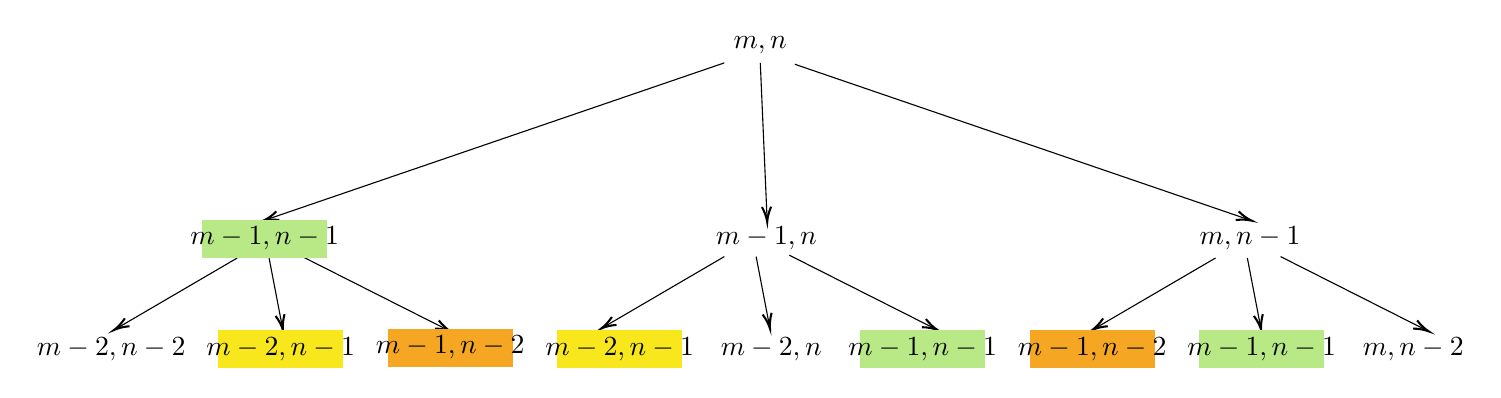
\begin{tikzpicture}[x=0.5pt,y=0.5pt,yscale=-1,xscale=1]
%uncomment if require: \path (0,284); %set diagram left start at 0, and has height of 284

%Straight Lines [id:da1383331413383435] 
\draw    (522.5,36) -- (191.39,149.35) ;
\draw [shift={(189.5,150)}, rotate = 341.1] [color={rgb, 255:red, 0; green, 0; blue, 0 }  ][line width=0.75]    (10.93,-3.29) .. controls (6.95,-1.4) and (3.31,-0.3) .. (0,0) .. controls (3.31,0.3) and (6.95,1.4) .. (10.93,3.29)   ;
%Straight Lines [id:da715204982720897] 
\draw    (548.5,36) -- (553.41,149) ;
\draw [shift={(553.5,151)}, rotate = 267.51] [color={rgb, 255:red, 0; green, 0; blue, 0 }  ][line width=0.75]    (10.93,-3.29) .. controls (6.95,-1.4) and (3.31,-0.3) .. (0,0) .. controls (3.31,0.3) and (6.95,1.4) .. (10.93,3.29)   ;
%Straight Lines [id:da8831806389031782] 
\draw    (573.5,37) -- (901.61,149.35) ;
\draw [shift={(903.5,150)}, rotate = 198.9] [color={rgb, 255:red, 0; green, 0; blue, 0 }  ][line width=0.75]    (10.93,-3.29) .. controls (6.95,-1.4) and (3.31,-0.3) .. (0,0) .. controls (3.31,0.3) and (6.95,1.4) .. (10.93,3.29)   ;
%Straight Lines [id:da6762777724306107] 
\draw    (170.5,177) -- (83.23,227.99) ;
\draw [shift={(81.5,229)}, rotate = 329.7] [color={rgb, 255:red, 0; green, 0; blue, 0 }  ][line width=0.75]    (10.93,-3.29) .. controls (6.95,-1.4) and (3.31,-0.3) .. (0,0) .. controls (3.31,0.3) and (6.95,1.4) .. (10.93,3.29)   ;
%Straight Lines [id:da9537842571445845] 
\draw    (193.5,177) -- (203.12,227.04) ;
\draw [shift={(203.5,229)}, rotate = 259.11] [color={rgb, 255:red, 0; green, 0; blue, 0 }  ][line width=0.75]    (10.93,-3.29) .. controls (6.95,-1.4) and (3.31,-0.3) .. (0,0) .. controls (3.31,0.3) and (6.95,1.4) .. (10.93,3.29)   ;
%Straight Lines [id:da25240177172893863] 
\draw    (217.5,176) -- (322.71,229.1) ;
\draw [shift={(324.5,230)}, rotate = 206.78] [color={rgb, 255:red, 0; green, 0; blue, 0 }  ][line width=0.75]    (10.93,-3.29) .. controls (6.95,-1.4) and (3.31,-0.3) .. (0,0) .. controls (3.31,0.3) and (6.95,1.4) .. (10.93,3.29)   ;
%Straight Lines [id:da4227912867383341] 
\draw    (522.5,176) -- (435.23,226.99) ;
\draw [shift={(433.5,228)}, rotate = 329.7] [color={rgb, 255:red, 0; green, 0; blue, 0 }  ][line width=0.75]    (10.93,-3.29) .. controls (6.95,-1.4) and (3.31,-0.3) .. (0,0) .. controls (3.31,0.3) and (6.95,1.4) .. (10.93,3.29)   ;
%Straight Lines [id:da490335830545392] 
\draw    (545.5,176) -- (555.12,226.04) ;
\draw [shift={(555.5,228)}, rotate = 259.11] [color={rgb, 255:red, 0; green, 0; blue, 0 }  ][line width=0.75]    (10.93,-3.29) .. controls (6.95,-1.4) and (3.31,-0.3) .. (0,0) .. controls (3.31,0.3) and (6.95,1.4) .. (10.93,3.29)   ;
%Straight Lines [id:da44453803269503656] 
\draw    (569.5,175) -- (674.71,228.1) ;
\draw [shift={(676.5,229)}, rotate = 206.78] [color={rgb, 255:red, 0; green, 0; blue, 0 }  ][line width=0.75]    (10.93,-3.29) .. controls (6.95,-1.4) and (3.31,-0.3) .. (0,0) .. controls (3.31,0.3) and (6.95,1.4) .. (10.93,3.29)   ;
%Straight Lines [id:da6159232694423369] 
\draw    (877.5,177) -- (790.23,227.99) ;
\draw [shift={(788.5,229)}, rotate = 329.7] [color={rgb, 255:red, 0; green, 0; blue, 0 }  ][line width=0.75]    (10.93,-3.29) .. controls (6.95,-1.4) and (3.31,-0.3) .. (0,0) .. controls (3.31,0.3) and (6.95,1.4) .. (10.93,3.29)   ;
%Straight Lines [id:da04820263440719896] 
\draw    (900.5,177) -- (910.12,227.04) ;
\draw [shift={(910.5,229)}, rotate = 259.11] [color={rgb, 255:red, 0; green, 0; blue, 0 }  ][line width=0.75]    (10.93,-3.29) .. controls (6.95,-1.4) and (3.31,-0.3) .. (0,0) .. controls (3.31,0.3) and (6.95,1.4) .. (10.93,3.29)   ;
%Straight Lines [id:da4987937509957987] 
\draw    (924.5,176) -- (1029.71,229.1) ;
\draw [shift={(1031.5,230)}, rotate = 206.78] [color={rgb, 255:red, 0; green, 0; blue, 0 }  ][line width=0.75]    (10.93,-3.29) .. controls (6.95,-1.4) and (3.31,-0.3) .. (0,0) .. controls (3.31,0.3) and (6.95,1.4) .. (10.93,3.29)   ;

% Text Node
\draw (548.38,23.47) node   [align=left] {$\displaystyle m,n$};
% Text Node
\draw  [color={rgb, 255:red, 184; green, 233; blue, 134 }  ,draw opacity=1 ][fill={rgb, 255:red, 184; green, 233; blue, 134 }  ,fill opacity=1 ][line width=0.75]   (145.88,149.97) -- (234.88,149.97) -- (234.88,175.97) -- (145.88,175.97) -- cycle  ;
\draw (190.38,162.97) node   [align=left] {$\displaystyle m-1,n-1$};
% Text Node
\draw (552.88,162.97) node   [align=left] {$\displaystyle m-1,n$};
% Text Node
\draw (902.38,162.97) node   [align=left] {$\displaystyle m,n-1$};
% Text Node
\draw (79.38,242.72) node   [align=left] {$\displaystyle m-2,n-2$};
% Text Node
\draw  [color={rgb, 255:red, 248; green, 231; blue, 28 }  ,draw opacity=1 ][fill={rgb, 255:red, 248; green, 231; blue, 28 }  ,fill opacity=1 ][line width=0.75]   (157.38,229.72) -- (246.38,229.72) -- (246.38,255.72) -- (157.38,255.72) -- cycle  ;
\draw (201.88,242.72) node   [align=left] {$\displaystyle m-2,n-1$};
% Text Node
\draw  [color={rgb, 255:red, 245; green, 166; blue, 35 }  ,draw opacity=1 ][fill={rgb, 255:red, 245; green, 166; blue, 35 }  ,fill opacity=1 ][line width=0.75]   (279.88,228.72) -- (368.88,228.72) -- (368.88,254.72) -- (279.88,254.72) -- cycle  ;
\draw (324.38,241.72) node   [align=left] {$\displaystyle m-1,n-2$};
% Text Node
\draw  [color={rgb, 255:red, 248; green, 231; blue, 28 }  ,draw opacity=1 ][fill={rgb, 255:red, 248; green, 231; blue, 28 }  ,fill opacity=1 ][line width=0.75]   (402.38,229.72) -- (491.38,229.72) -- (491.38,255.72) -- (402.38,255.72) -- cycle  ;
\draw (446.88,242.72) node   [align=left] {$\displaystyle m-2,n-1$};
% Text Node
\draw (556.38,242.72) node   [align=left] {$\displaystyle m-2,n$};
% Text Node
\draw  [color={rgb, 255:red, 184; green, 233; blue, 134 }  ,draw opacity=1 ][fill={rgb, 255:red, 184; green, 233; blue, 134 }  ,fill opacity=1 ][line width=0.75]   (621.38,229.72) -- (710.38,229.72) -- (710.38,255.72) -- (621.38,255.72) -- cycle  ;
\draw (665.88,242.72) node   [align=left] {$\displaystyle m-1,n-1$};
% Text Node
\draw  [color={rgb, 255:red, 245; green, 166; blue, 35 }  ,draw opacity=1 ][fill={rgb, 255:red, 245; green, 166; blue, 35 }  ,fill opacity=1 ][line width=0.75]   (743.88,229.72) -- (832.88,229.72) -- (832.88,255.72) -- (743.88,255.72) -- cycle  ;
\draw (788.38,242.72) node   [align=left] {$\displaystyle m-1,n-2$};
% Text Node
\draw  [color={rgb, 255:red, 184; green, 233; blue, 134 }  ,draw opacity=1 ][fill={rgb, 255:red, 184; green, 233; blue, 134 }  ,fill opacity=1 ][line width=0.75]   (866.38,229.72) -- (955.38,229.72) -- (955.38,255.72) -- (866.38,255.72) -- cycle  ;
\draw (910.88,242.72) node   [align=left] {$\displaystyle m-1,n-1$};
% Text Node
\draw (1020.38,242.72) node   [align=left] {$\displaystyle m,n-2$};


\end{tikzpicture}

}
\caption{A directed graph and its two shortest path trees. The array representation
for the first tree is $prev[s,a,b,c,f,h,j,k] = [null, s, a, f, s, c, c, b]$.}
\label{fig:tree}
\end{figure}


%\subsection*{Determining Shortest Path Tree}

We now modify the three algorithms, BFS, Dijkstra's algorithm, and Bellman-Ford algorithm, to allow them to generate a shortest path tree.
The idea is that, %to keep track of its predecessor of each vertex~(essentially the parent of $v$ in the shortest path tree).
%We use array $prev$ of size $|V|$ to do it.
whenever $dist[v]$ gets updated as $dist[u] + l(u,v)$ we also immediately assign $prev[v]$ as $u$.
See their pseudo-codes below.

\begin{minipage}{0.8\textwidth}
	\aaA {17}{Algorithm BFS~($G = (V, E), s \in V$)}\xxx
	\aab {$dist[v] = \infty$, for any $v\in V$;}\xxx
	\aab {\textcolor{blue}{$prev[v] = null$, for any $v\in V$};}\xxx
	\aab {init an empty queue $Q$;}\xxx
	\aab {$dist[s] = 0$;}\xxx
	\aab {insert~($Q, s$);}\xxx
	\aaB {9}{while~(empty~($Q$) = false)}\xxx
	\aac {$u$ = find-earliest~($Q$);}\xxx
	\aac {delete-earliest~($Q$);}\xxx
	\aaC {5}{for each edge~$(u, v)\in E$}\xxx
	\aaD {4}{if~($dist[v] = \infty$)}\xxx
	\aae {$dist[v] = dist[u] + 1$;}\xxx
	\aae {\textcolor{blue}{$prev[v] = u$;}}\xxx
	\aae {insert~($Q$, $v$);}\xxx
	\aad {end if;}\xxx
	\aac {end for;}\xxx
	\aab {end while;}\xxx
	\aaa {end algorithm;}\xxx
\end{minipage}


\begin{minipage}{0.8\textwidth}
	\aaA {18}{Algorithm Dijkstra~($G = (V, E)$, $l(e)$ for any $e\in E$, $s \in V$)}\xxx
	\aab {$dist[v] = \infty$, for any $v\in V$;}\xxx
	\aab {\textcolor{blue}{$prev[v] = null$, for any $v\in V$};}\xxx
	\aab {init an empty priority queue $PQ$;}\xxx
	\aab {for any $v\in V$: insert~($PQ$, $v$), where the priority of $v$ is $\infty$;}\xxx
	\aab {$dist[s] = 0$;}\xxx
	\aab {decrease-key~($PQ, s, 0$);}\xxx
	\aaB {10}{while~(empty~($PQ$) = false)}\xxx
	\aac {$u$ = find-min~($PQ$);}\xxx
	\aac {delete-min~($PQ$);}\xxx
	\aaC {6}{for each edge~$(u, v)\in E$}\xxx
	\aaD {4}{if~($dist[v] > dist[u] + l(u,v)$)}\xxx
	\aae {$dist[v] = dist[u] + l(u,v)$;}\xxx
	\aae {\textcolor{blue}{$prev[v] = u$;}}\xxx
	\aae {decrease-key~($PQ$, $v$, $dist[v]$);}\xxx
	\aad {end if;}\xxx
	\aac {end for;}\xxx
	\aab {end while;}\xxx
	\aaa {end algorithm;}\xxx
\end{minipage}

\begin{minipage}{0.8\textwidth}
	\aaA {9}{Algorithm Bellman-Ford~($G = (V, E)$, $l(e)$ for any $e\in E$, $s \in V$)}\xxx
	\aab {init an array $dist$ of size $|V|$;}\xxx
	\aab {$dist[s] = 0$; $dist[v] = \infty$ for any $v\neq s$;}\xxx
	\aab {\textcolor{blue}{$prev[v] = null$, for any $v\in V$};}\xxx
	\aaB {4}{for $k = 1 \to |V| - 1$}\xxx
	\aaC {2}{for each edge $(u,v)\in E$}\xxx
	\aad {$update(u,v)$;}\xxx
	\aac {end for;}\xxx
	\aab {end for;}\xxx
%	\aab {report: $dist[v]$ gives $distance(s,v)$, for any $v\in V$;}\xxx
	\aaa {end algorithm;}\xxx
\end{minipage}

\begin{minipage}{0.8\textwidth}
	\aaA {5}{procedure update~(edge $(u,v)\in E$)}\xxx
	\aaB {3}{if~($dist[v] > dist[u] + l(u,v)$)}\xxx
	\aac {$dist[v] = dist[u] + l(u,v)$;}\xxx
	\aac {\textcolor{blue}{$prev[v]= u$};}\xxx
	\aab {end if;}\xxx
	\aaa {end procedure;}\xxx
\end{minipage}


The resulting $prev$ array corresponds to a graph called $T$, in which the vertices are $V$
and edges are $\{(prev[v], v)\mid v\in V\}$. We now prove that this graph is indeed one shortest path tree,
by showing $T$ satisfying the 4 conditions in the definition. It is trivial to verify that the conditions (2)
is satisfied, as the vertices are $V$; condition (3) is easy as well, as in any of the algorithm,
assigning $u$ to $prev[v]$ already happens when examining edge $(u,v)\in E$.
Below we then prove condition (1) and (4).

\begin{fact}
\label{tree-fact2}
At any time of the algorithm, for any $v\in V$, let $u = prev[v]$, if $u\neq null$ then $dist[v] = dist[u] + l(u,v)$;
in particular, when the algorithm terminates, we have $distance(s,v) = distance(s,u) + l(u,v)$.
\end{fact}
The first part of above fact is a direct consequence of each algorithm as we update $prev$ right after updating $dist[v]$ as $dist[u] + l(u,v)$.
The secon part also uses the correctness of each algorithm, i.e., when each algorithm terminates, we have $dist[v] = distance(s,v)$.

We now prove condition (1), i.e., $T$ is a tree with root being $s$~(although we use $T$ but we have not showed that it is a tree).
Since $T$ corresponds to array $prev$, it is obvious that in-degree of $s$ is 0 and that each vertex in $T$, except $s$,
has in-degree of 1. We therefore just need to prove that $T$ does not contain cycle. 
We need a stronger assumption to make it true. That is, the graph $G$ cannot contain negative nor length-zero cycles.

\begin{fact}
$T$ does not contain cycle, if all cycles in $G$ are of positive length.
\end{fact}
\emph{Proof.} Suppose conversely that there exists a cycle $C = v_1\to v_2\to \cdots \to v_k\to v_1$ in $T$.
Following above fact, we have $dist[v_i] = dist[v_{i-1}] + l(v_{i-1},v_i)$, for every $1 < i \le k$
and $dist[v_1] = dist[v_k] + l(v_k,v_1)$.
Summing up both sides gives $\sum_{e\in C} l(e) = 0$, contradicting to the the assumption
that all cycles have positive length.\qed

Last, we prove condition (4):
\begin{claim}
For every $v\in V$, the unique path from $s$ to $v$ in $T$ is one shortest path from $s$ to $v$ in $G$,
if all cycles in $G$ are positive cycles.
\end{claim}
\emph{Proof.} 
Let $p: s = v_0 \to v_1 \to v_2 \to \cdots \to v_k$ be the path from $s$ to $v_k$ in $T$.
By the construction of $T$, we know that $prev[v_i] = v_{i - 1}$, $1\le i \le k$.
Therefore, using Fact~\ref{tree-fact2}, we have $distance(s, v_i) = distance(s, v_{i-1}) + l(v_{i-1}, v)$,
for each $i = 1, 2, \cdots, k$. We sum up the left side and the right side of these $k$ equations.
Canceling out $distance(s, v_i)$, $i = 1, 2, \cdots, k-1$, on both sides gives
$distance(s,v_k) = distance(s, s) + \sum_{i=1}^k l(v_{i-1}, v_i) = \sum_{i=1}^k l(v_{i-1}, v_i)$, implying that
the length of $p$ is equal to the distance from $s$ to $v_k$, i.e., it is one shortest path from $s$ to $v_k$. \qed


